\documentclass[a4paper,twocolumn]{article}

\usepackage[english]{babel}
\usepackage[utf8]{inputenc}
\usepackage{graphicx}
\usepackage{hyperref}
\usepackage{amsmath}
\usepackage{amssymb}
\usepackage{amsbsy}

\usepackage[cm]{fullpage}
\usepackage[small]{titlesec}
% patch titlesec bug of not showing (sub)title numbering http://tex.stackexchange.com/a/300259
\usepackage{etoolbox}
\makeatletter
\patchcmd{\ttlh@hang}{\parindent\z@}{\parindent\z@\leavevmode}{}{}
\patchcmd{\ttlh@hang}{\noindent}{}{}{}
\makeatother

\let\originalleft\left
\let\originalright\right
\renewcommand{\left}{\mathopen{}\mathclose\bgroup\originalleft}
\renewcommand{\right}{\aftergroup\egroup\originalright}

\usepackage{amssymb}
\renewcommand{\H}{\mathcal{H}}
\newcommand{\N}{\mathcal{N}}
\renewcommand{\L}{\mathcal{L}}
\renewcommand{\O}{\mathcal{O}}
\newcommand{\Lhybrid}{\L_{\mathtt{hybrid}}}
\newcommand{\Ldisc}{\L_{\mathtt{disc}}}
\newcommand{\Lgen}{\L_{\mathtt{gen}}}

\let\originalnu\nu
\renewcommand{\nu}{\boldsymbol{\originalnu}}


\title{Online Incremental Feature Learning with Denoising Autoencoders$-$ summary}
\author{Matěj Nikl}

\begin{document}
\maketitle
\noindent
Determining the optimal model complexity, i.e. the number of features for DAE is a nontrivial problem. Moreover, in large-scale and online datasets the cross-validation method enabling the hyper-parameter search is even more challenging.

This adaptive feature learning algorithm tries to address the given issue by:
\begin{enumerate}
    \item adding and training new features to minimize the residual of the objective function
    \item merging similar features to avoid redundant feature representations
\end{enumerate}
Having a variable number of features gives the model the ability to make itself more/less complex according to the (even changing) dataset needs.

\section{Denoising Autoencoder}
The standard Denoising Autoencoder is used as a building block for incremental feature learning, it consists of four components:
\begin{itemize}
    \item a conditional distribution $q(\mathbf{\widetilde{x}|x})$, that corrupts $\mathbf{x}$ into $\mathbf{\widetilde{x}}$
    \item an encoding function $f(\mathbf{\widetilde{x}}) = \sigma(\mathbf{W\widetilde{x} + b}) \equiv \mathbf{h} \in \mathbb{R}^N$, which gives a representation of input data $\mathbf{x}$
    \item an decoding function $g(\mathbf{h}) = \sigma(\mathbf{W}^T\mathbf{h + c}) \equiv \mathbf{\widehat{x}} \in \mathbb{R}^D$, which recovers the data from the representation $\mathbf{h}$
    \item a differentiable (cross-entropy) cost function $\L(\mathbf{x}) = \H(\mathbf{x}, \mathbf{\widehat{x}}) \in \mathbb{R}$, which computes the dissimilarity between input and reconstruction
\end{itemize}

\section{Incremental Feature Learning}
The incremental feature learning algorithm needs to address the following problems:
\begin{enumerate}
    \item \textbf{when} to add and merge features
    \item \textbf{how} to add and merge features
\end{enumerate}
In order to deal with these problems, the authors have chosen the following procedure:
\begin{enumerate}
    \item form a set $B$ of hard training examples: $B \leftarrow B \cup \{\textbf{x}\}$ if $\L(\textbf{x}) > \mu$, which is used to greedily train the new features
    \item merge similar + add new features when there are enough examples in $B$: $|B| > \tau$
\end{enumerate}
I.e. when there is enough \textit{hard} examples, $2\Delta M$ old features are merged into $\Delta M$ new features, $\Delta N$ new features are simply added, and these new features are greedily trained on the set $B$ of hard training examples. After convergence, set $B = \emptyset$ and continue standard training of all features.

In this paper $\mu$ was set as average of the objective function for recent $10000$ examples, $\tau$ was also set as 10000.

\paragraph{Notations.} $D$ denotes input dimension, $N$ the number of (existing) features, and K the number of class labels. The parameters for generative training are defined as the (tied) weight matrix $\mathbf{W} \in \mathbb{R}^{N \times D}$, the hidden bias $\mathbf{b} \in \mathbb{R}^N$, and the input bias $\mathbf{c} \in \mathbb{R}^D$. Similarly, the parameters for discriminative training are composed of the weight matrix $\mathbf{\Gamma} \in \mathbb{R}^{K \times N}$ between hidden and output units, the output bias $\nu \in \mathbb{R}^K$, as well as the weight matrix $\mathbf{W}$ and the hidden bias $\mathbf{b}$. $\N$ is used to denote \textit{new} features and $\O$ to denote existing or \textit{old} features, thus $\theta_\O = \{\mathbf{W_\O, b_\O, c, \Gamma_\O, \nu}\}$, and $\theta_\N = \{\mathbf{W_\N, b_\N, c, \Gamma_\N, \nu}\}$.

\begin{figure*}[t]
    \centering
    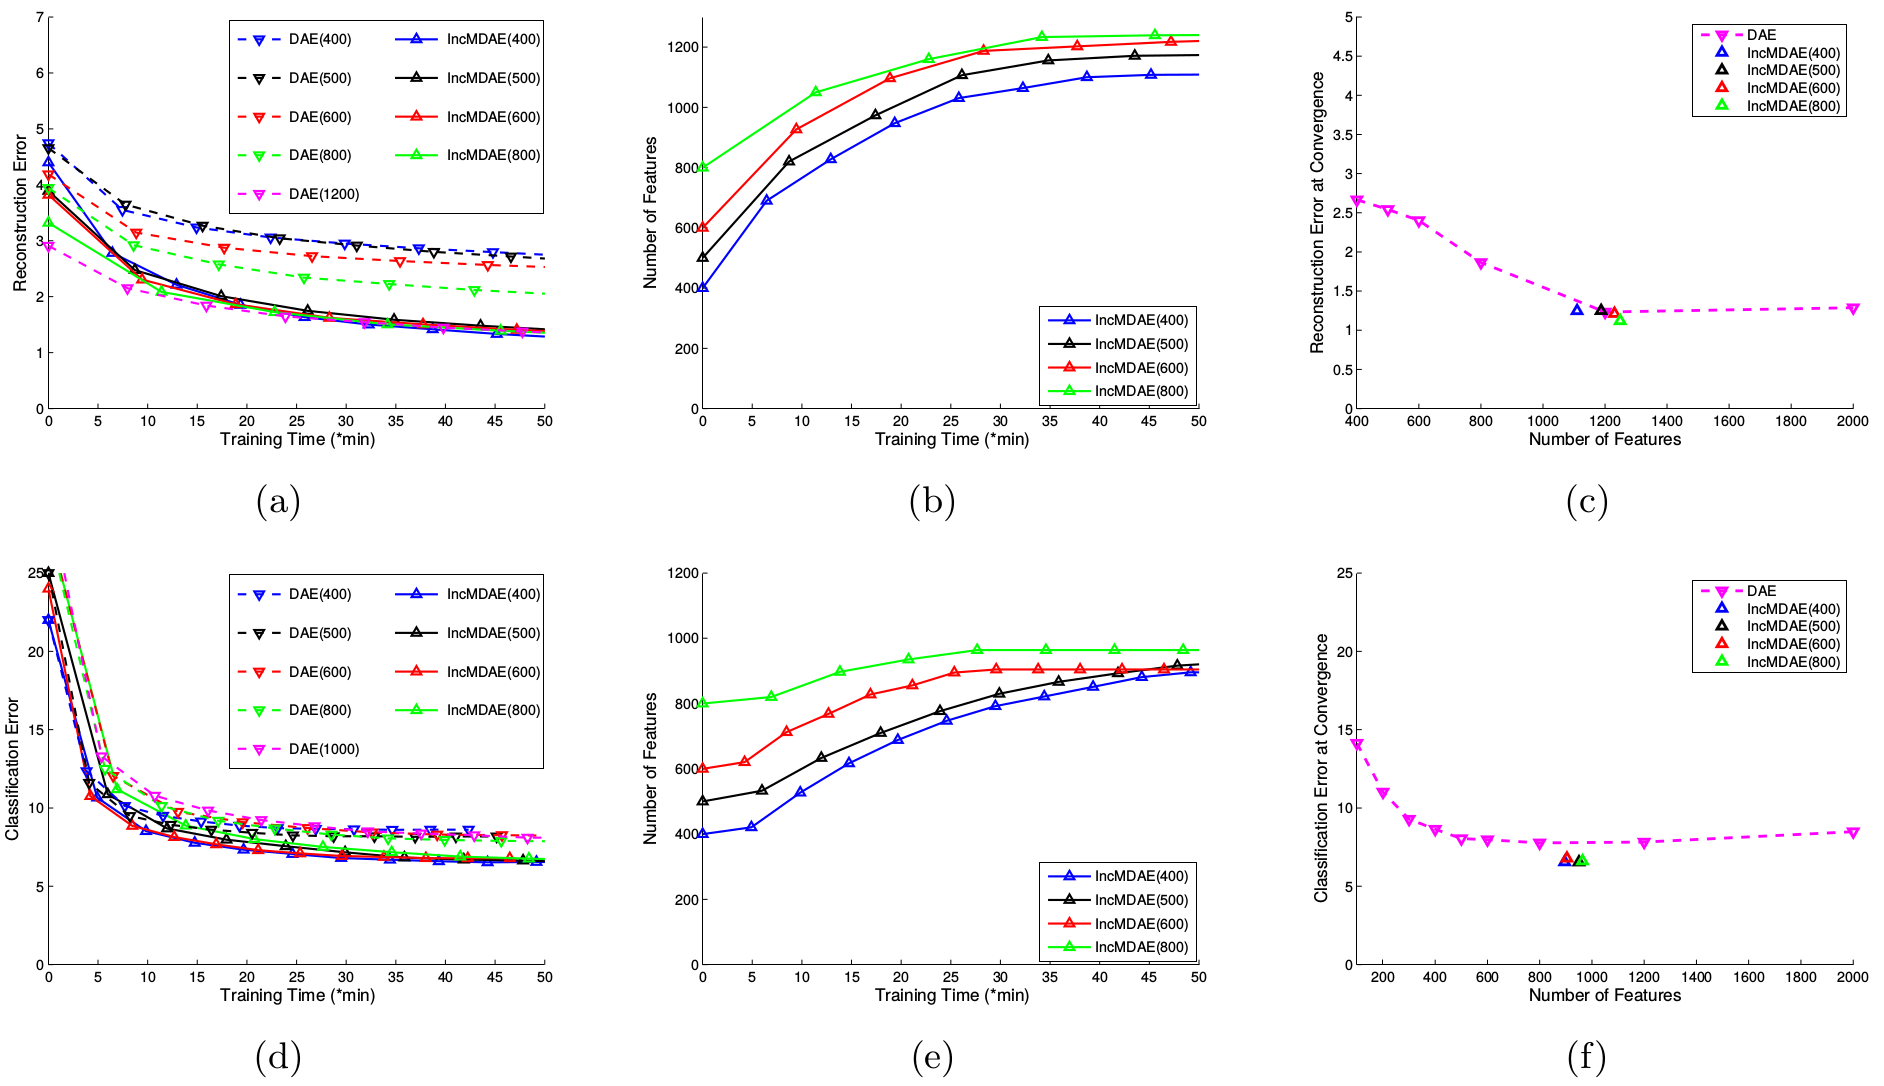
\includegraphics[width=0.9\textwidth]{graph.png}
    \caption{(a,d) Test (online) reconstruction error and classification error of incremental (IncMDAE) and non-incremental DAE. (b,e) The number of features for incremental learning with generative and hybrid criteria. (c,f) Test reconstruction error and classification error at convergence. The numbers in parentheses refer to the initial number of features.}
    \label{fig:graph}
\end{figure*}

\subsection{Adding Features} \label{ssec:adding}
New features are being added and trained upon, whenever there is enough examples in the \textit{hard set} $B$.
The basic idea for efficient training is that only the new features $\theta_\N$ are trained to minimize the objective function while keeping $\theta_\O$ fixed.

\subsubsection{Generative Objective Function}
Measures reconstruction error between the input $\mathbf{x}$ and the reconstruction $\mathbf{\widehat{x}}$:
\begin{equation}
    \Lgen(\mathbf{x}) = \H(\mathbf{x}, \mathbf{\widehat{x}})
\end{equation}
The encoding and decoding functions for the new features can be written as:
\begin{align}
    \mathbf{h}_\N &= sigm(\mathbf{W_\N \widetilde{x}} + \mathbf{b_\N}) \\
 \label{equ:dec}
    \mathbf{\widehat{x}} &= sigm(\mathbf{W}_\N^T\mathbf{h}_\N + \mathbf{W}_\O^T\mathbf{h}_\O + \mathbf{c})
\end{align}
Moreover, since $\theta_\O$ is fixed, equation \eqref{equ:dec} can be rewritten to:
\begin{equation}
    \mathbf{\widehat{x}} = sigm(\mathbf{W}_\N^T\mathbf{h}_\N + c_d(\mathbf{h}_\O))
\end{equation}
where $c_d(\mathbf{h}_\O) \equiv \mathbf{W}_\O^T\mathbf{h}_\O + \mathbf{c}$ is viewed as a \textit{dynamic} decoding bias.
This allows for a efficient way of training new features, because $c_d(\mathbf{h}_\O)$ can be computed for each training example only once and then recalled without additional computational cost.

\subsubsection{Discriminative Objective Function}
Computes a classification loss between the actual label $\mathbf{y}$ and the predicted label $\mathbf{\widehat{y}}$:
\begin{gather}
    \Ldisc(\mathbf{x}, \mathbf{y}) = \H(\mathbf{y}, \mathbf{\widehat{y}}(\mathbf{x})) \\
    \mathbf{\widehat{y}} = \mathrm{softmax}(\mathbf{\Gamma_\N}f_\N(\mathbf{\widetilde{x}}) + \mathbf{\Gamma_\O}f_\O(\mathbf{\widetilde{x}}) + \nu)
\end{gather}
A similar interpretation for $\mathbf{\Gamma_\O}f_\O(\mathbf{\widetilde{x}}) + \nu$, as in the generative training is possible, and therefore, the new parameters $\{\mathbf{W_\N, b_\N, \Gamma_\N}\}$ can be trained efficiently as well.

\subsubsection{Hybrid Objective Function}
The proposed objective function for training new features is a linear combination of a generative and a discriminative objective function, called a \textit{hybrid} objective function:
\begin{equation}
    \Lhybrid = \Ldisc(\mathbf{x}, \mathbf{y}) + \lambda\Lgen(\mathbf{x})
\end{equation}
The values $\lambda \in [0.1, 0.4]$ gave roughly the best performance.

\subsection{Merging Features} \label{ssec:merging}
As a counterpart to the feature adding is the process of \textit{merging} the features, because only adding would lead to redundant features and overfitting.
Feature merging is done in two steps:
\begin{itemize}
    \item select a pair of candidate features to be merged, $\mathcal{M} = \{m_1, m_2\} \subset \O$, whose cosine distance $d(\textbf{W}_{m_1}, \textbf{W}_{m_2})$ is minimal, and replace $f_\O$ by $f_\O \setminus \mathcal{M}$
    \item add a new feature mapping $f_\N$ that \textit{replaces} the merged features, while initializing it as a weighted average of the selected two for faster convergence:
\end{itemize}
\begin{equation}
    \theta_\N = \frac{\sum_{\mathbf{x} \in B} P(h_{m_1}|\mathbf{x};\theta_{m_1})\theta_{m_1} + P(h_{m_1}|\mathbf{x};\theta_{m_2})\theta_{m_2}}
    {\sum_{\mathbf{x} \in B} P(h_{m_1}|\mathbf{x};\theta_{m_1}) + P(h_{m_1}|\mathbf{x};\theta_{m_2})}
\end{equation}

\subsection{Selecting $\Delta N$ and $\Delta M$}
Some kind of metric must be used to control the number of features being merged ($2\Delta M$) and added ($\Delta N$). A combination of AIC and BIC was used by authors, however the performance was fairly robust to the choice of update rule for $\Delta N$ and $\Delta M$.

\section{Principles of modularization}
Individual hidden units are treated as modules $-$ they are being manipulated (added and merged), however this does not allow for any kind of modular-like design for multi-task setting.

\section{Principles of growing}
This kind of architecture is well capable of growing (and shrinking), as explained in \ref{ssec:adding} and \ref{ssec:merging}, however it only increases or decreases the model's complexity (and allows to adapt faster to e.g. changing distribution of the dataset during online training).


\end{document}
